\documentclass[journal,article,submit,oneauthor,pdftex,10pt,a4paper,games]{mdpi} 

\firstpage{1} 
\makeatletter 
\setcounter{page}{\@firstpage} 
\makeatother 
\articlenumber{x}
\doinum{10.3390/------}
\pubvolume{xx}
\pubyear{2017}
\copyrightyear{2017}
\externaleditor{Academic Editor: name}
\history{Received: date; Accepted: date; Published: date}

% import of libraries
\usepackage{algorithm}
\usepackage{algpseudocode}
\usepackage{mathtools}
\usepackage{tikz}
\usepackage{listings}
\usepackage{pgfplots}
\usepackage{color}
\usepackage{subcaption}
\usepackage{mathdots}
\usepackage{hyperref}

% configuration of libraries
\usetikzlibrary{arrows,automata}
\usetikzlibrary{positioning}
\tikzset{
    state/.style={
           rectangle,
           rounded corners,
           draw=black, very thick,
           minimum height=2em,
           inner sep=2pt,
           text centered,
           },
}
\lstset{language=Python}
\pgfplotsset{width=10.5cm,compat=1.8}
\makeatletter

% newcommand for inline equations used in appendices
\newcommand*{\inlineequation}[2][]{
  \begingroup
    \refstepcounter{equation}
    \ifx\\#1\\
    \else
      \label{#1}
    \fi
    \relpenalty=10000
    \binoppenalty=10000
    \ensuremath{
      #2
    }
    ~\@eqnnum
  \endgroup
}
\makeatother



\Title{Non-Markov Stateful Evolutionary Games}
\Author{}
\AuthorNames{}
\address[1]{
 \quad }

\abstract{A new evolutionary game is introduced which incorporates states and actions into the strategies of the organisms of the evolving populations. The game centrally features actions that result in demographic flow between states that may not conserve organism numbers. It is by this feature that the game encapsulate a range of other evolutionary games, and can encode almost very complex interactions between organisms, species and populations.
The game's formalism is expounded and the nature of the game's equilibrium is discussed. This discussion leads to an algorithm for numerically determining the stable equilibrium points which is exemplified in the context of a modified Hawk-Dove game. The game's flexibility for modeling population dynamics is evaluated and compared with other evolutionary games.}
\keyword{Evolutionary stable strategies (ESS); Markov decision evolutionary games (MDEG); Hawk-Dove game; Evolutionary dynamics; Evolutionary Game Theory}

% not sure if I should include these or not?
%\PACS{02.50.Le}
%\MSC{91A22}
%\JEL{C73}


\datasetlicense{CC-BY}
\begin{document}


\section{Introduction}
Biological species are well recognised as being engaged in an evolutionary fight-for-survival and Game Theory has been used to analyse the strategies in such a fight.
This kind of analysis is the defining feature of Evolutionary Game Theory, whose many features and concepts are often credited to John Maynard Smith and George R. Price \cite{maynard,maynard2}.
The most standard evolutionary game concerns the continuous growth/decay of organism types; the organism types are defined by the strategy they play as they are continuously randomly paired to participate in a simultaneous symmetric two-player game where the expected payoff determines each participant's growth.\cite{weibull}
However, there is sometimes felt to be a component missing from evolutionary analysis of strategies - the consideration of state.\cite{socialpsyc1,errors1}

Evolutionary game theory has been a valuable tool in characterising the dynamics and interactions among biological species and it also has proven utility in other fields which feature evolutionary dynamics.  Some examples of phenomena which have been modeled via Evolutionary Game Theory include: altruism, empathy, human culture, moral behavior, private property, proto-linguistic behavior, social learning, societal norms, personality and mating-dynamics \cite{sep-game-evolutionary,socialpsyc1,Hodgson2012,McNamara953}.

However, many organisms exhibit behaviors and strategies which are intrinsically coupled with state and hence cannot be directly modeled using standard evolutionary game theory.
Simple and canonical examples include the behavior of perspiring with increasing body temperature causing dehydration, foraging behavior with hunger signals causing food shortage, sleep with ambient light levels causing vulnerability to predation, or hibernation with the change of season causing hunger.

Within this paper we detail an evolutionary game for modeling stateful evolutionary dynamics and an algorithm which solves for its equilibria. We give a simple demonstration of the game via an extension of the classic Hawk-Dove game\cite{maynard} and we compare the game with the approach of others.

\subsection{Related Work}
Complex state-action interactions between individuals can always be stochastically modeled by artificial life simulations.\cite{alife1} But recent work has been conducted to incorporate some state-action dynamics into the exacting mathematical framework of evolutionary game theory.

This work has developed along two different branches, the first branch consists of encoding the organisms as belonging to nodes on a graph structure.\cite{spacial4} In this approach the organisms at a node play the symmetric game against weighted probabilities of their nearest neighbors and/or themself. Such games are called `Spacial Evolutionary Games'\cite{spacial1,nowak} and they have unique and dynamic behavior\cite{spacial2,spacial3}. Spacial Evolutionary Games feature the addition of specifying a `who-plays-with-who' into the game structure but the game itself is the same for all the participants.
Spacial Evolutionary Games are apt to model the evolution of organism's strategies between strategic nodes but it is seen to fail to capture the organisms having state beyond generalised location.

The second approach is more recent and consists of integrating state (and transitions between state) into the symmetric two-player game itself. This pioneering effort has centered around the works of Eitan Altman, and his colleagues Ilaria Brunetti and Yezekael Hayel \cite{markov2,markov3,markov4,markov5,markov8,markov9}, who introduce the Markov-Decision-Evolutionary-Game (MDEG) and variants thereof.

An MDEG consists in analysing the growth/decay of organism-types in a population where the organisms can occupy a finite set of states. The organism-types are defined by the strategy they play of choosing actions depending on their state as they are continuously randomly paired to participate in a two-player symmetric game. The game consists of each participant choosing an action and the game's outcomes depend on the chosen actions and the states of the participants. The game's outcomes determine the instantaneous payoff and probable transition to other states experienced by the participants. The expected long-term payoff determines the growth/decay of the organism-types which then changes the composition of the population in which the game is played.

Several example MDEG games are introduced in Altman's literature including modifications and extensions of the Hawk-Dove game from which we take inspiration.\cite{markov3,markov5}
MDEG includes many features for modeling state-action interactions within evolutionary game theory and serves to provide a contrast for our game. By our game, we show that by relaxing the markov nature of MDEG we allow a remarkably more flexible game, a game which features other evolutionary games as subtypes.

\subsection{Structure}
The remainder of this paper is organised as follows: section \ref{sec:2} presents the core concept of non-markovian transmission of organisms between states, section \ref{section:formalism} gives formalism to the non-markovian game and its algorithm, section \ref{sec:equilibria} discusses the game's equilibria and gives confinement for the algorithm's equilibria search, section \ref{sec:example} details a Hawk-Dove game as example of the working algorithm, and section \ref{sec:discussion} concludes the paper by evaluating and comparing the features of our game.

\section{Non-Markov population models}\label{sec:2}

The demographic flow of individuals of a species' population between states is sometimes described in ecological-studies by a matrix that is not necessarily markov.\cite{population1}
The simplest example of such matrices are Leslie Matrices used for studying the structure of populations of individuals transitioning between evenly spaced age-states.
Leslie Matrices are square, and they have form \cite{leslie}:

\begin{equation*}
M=\begin{bmatrix}
    F_0 & F_1 & F_2 & \dots  & F_{m-2} & F_{m-1} & F_m  \\
    P_0 &  0  &  0  & \dots  &    0    &  0      &  0   \\
     0  & P_1 &  0  & \dots  &    0    &  0      &  0   \\
     0  &  0  & P_2 & \dots  &    0    &  0      &  0   \\
    \vdots & \vdots & \vdots & \ddots & \vdots & \vdots & \vdots \\
     0  &  0  &  0  & \dots  & P_{m-2} &  0      &  0   \\
     0  &  0  &  0  & \dots  &    0    & P_{m-1} &  0   \\
\end{bmatrix}
~~~0<P_x<1;~~F_x\ge0
\end{equation*}
Where $P_i$ represents the probability of and individual in the $i$th age bracket successfully living into the $(i+1)$th age bracket, and $F_i$ is average number of offspring for an individual in $i$th age bracket within the duration of the age bracket.
For a column vector $n = [n_0,n_1,n_2,\dots,n_m]$ with each $n_i$ representing the number of individuals in each age-bracket, $Mn$ gives the expected number of individuals in the population after the duration of one age bracket of time, and $M^2n$ the expectation individuals after two age brackets, $M^3n$ after three, and so on.
Successive applications eventually yield a steady population profile between the $n_i$, and a constant exponential growth rate $\lambda$ given by the Euler–Lotka equation.
The $\lambda$ is the dominant and only real-positive eigenvalue of the matrix, with the steady distribution $n$ as its corresponding eigenvector, that is $Mn=\lambda n$.

Although the elements in the Leslie matrix are positive and represent states of organisms in the population and the transition between, the matrix isn't Markov because its columns don't necessarily sum to one.  The informal difference is that whereas in a Markov-chain matrix the elements represent the expectation of \textit{transition} between states, Leslie matrix elements represent the expectation of \textit{transmission} between states inclusive of such possible factors as births and deaths.
We term the class of such matrices as `transmission matrices' in this article and assert the only thing defining such matrices are that they are real, square and have non-negative elements.\footnote{General non-negative real square matrices (or at-least irreducible ones) have at-least one real non-negative eigenvalue (via indirect application of Perron-Frobenius theorem, see chapter 3 of \cite{matrix2}) hence a transmission matrix identifies at-least one growth-rate}
We do this because such matrices can be built more broadly than simple Leslie-matrix form\cite{models1,models2}. Consider the rich interaction between organism-states captured by the matrix of transmissions for the 'Nodding Thistle' in figure \ref{fig:1}.



\begin{figure}[h]
    \begin{subfigure}[b]{.5\linewidth}
        \centering
        \begin{tikzpicture}[scale=0.9, transform shape,->,>=stealth',shorten >=1pt,auto,node distance=1.7cm,thick,main node/.style={circle}]
            \path[use as bounding box] (-2.5cm, -2.8cm) rectangle (2.5cm, 2.5cm);
            \node[main node] (SB)  at (-2cm,  2cm) [align=center, text width=2.1cm] {\includegraphics[width=.05\textwidth]{1.png}\\\small Seed};
            \node[main node] (SM)  at ( 2cm,  2cm) [align=center, text width=2.1cm] {\includegraphics[width=.25\textwidth]{2.png}\\\small Small};
            \node[main node] (ME)  at ( 2cm, -2cm) [align=center, text width=2.1cm] {\includegraphics[width=.29\textwidth]{3.png}\\\small Medium};
            \node[main node] (LE)  at (-2cm, -2cm) [align=center, text width=2.1cm] {\includegraphics[width=.38\textwidth]{4.png}\\\small Large};

            \node[main node] (SBm) at (-2cm,  2cm) [align=center, text width=1.2cm] {};
            \node[main node] (SMm) at ( 2cm,  2cm) [align=center, text width=1.2cm] {};
            \node[main node] (MEm) at ( 2cm, -2cm) [align=center, text width=1.2cm] {};
            \node[main node] (LEm) at (-2cm, -2cm) [align=center, text width=1.2cm] {};

            \path[every node/.style={sloped,auto=false}]
            (SBm) edge [in=180-20,out=180+20,looseness=3,   line width=1pt,anchor=south] node  {\scriptsize 0.443} (SBm)
            (SBm) edge [bend left=15,                       line width=1pt,anchor=south] node  {\scriptsize 0.0039} (SMm)
            (SBm) edge [bend left=15,                       line width=1pt,anchor=south] node  {\scriptsize 0.0004} (MEm)
            (SBm) edge [bend left=15,                       line width=1pt,anchor=south] node  {\scriptsize 0.0005} (LEm)

            (SMm) edge [bend left=15,                       line width=1pt,anchor=south] node  {\scriptsize 0.1584} (SBm)
            (SMm) edge [in=20,out=-20,looseness=3,          line width=1pt,anchor=north] node  {\scriptsize 0.0078} (SMm)
            (SMm) edge [bend left=15,                       line width=1pt,anchor=south] node  {\scriptsize 0.0031} (MEm)
            (SMm) edge [bend left=15,                       line width=1pt,anchor=north] node  {\scriptsize 0.01} (LEm)

            (MEm) edge [bend left=15,                       line width=1pt,anchor=north] node  {\scriptsize 6.6105} (SBm)
            (MEm) edge [bend left=15,                       line width=1pt,anchor=south] node  {\scriptsize 0.2434} (SMm)
            (MEm) edge [in=-20,out=20,looseness=3,          line width=1pt,anchor=south] node  {\scriptsize 0.0314} (MEm)
            (MEm) edge [bend left=15,                       line width=1pt,anchor=south] node  {\scriptsize 0.0613} (LEm)

            (LEm) edge [bend left=15,                       line width=1pt,anchor=south] node  {\scriptsize 206.56} (SBm)
            (LEm) edge [bend left=15,                       line width=1pt,anchor=south] node  {\scriptsize 7.6091} (SMm)
            (LEm) edge [bend left=15,                       line width=1pt,anchor=south] node  {\scriptsize 0.793} (MEm)
            (LEm) edge [in=180+20,out=180-20,looseness=3,   line width=1pt,anchor=north] node  {\scriptsize 0.945} (LEm)
            ;
        \end{tikzpicture}

        \caption{Life cycle graph of the population model}\label{fig:1a}
    \end{subfigure}
    \begin{subfigure}[b]{.5\linewidth}
        \centering
        \footnotesize
        $$ \begin{bmatrix}\text{Seed}_{t+1}\\\text{Small}_{t+1}\\\text{Medium}_{t+1}\\\text{Large}_{t+1}\end{bmatrix}= 
        \begin{bmatrix}
            0.443&0.1584&6.6105&206.56\\
            0.039&0.0078&0.2434&7.6091\\
            0.0004&0.0031&0.0314&0.793\\
            0.0005&0.01&0.0613&0.945
        \end{bmatrix}
        \begin{bmatrix}\text{Seed}_{t}\\\text{Small}_{t}\\\text{Medium}_{t}\\\text{Large}_{t}\end{bmatrix}$$
        \caption{
            4x4 matrix model of a Nodding Thistle (\textit{Carduus nutans}) population in Australia, classification based on seed and rosette size. The transmission numbers represent aggregate survival/growth/propagation of individuals from one class into another per year. The projected population growth rate ($\lambda$) is 1.207 per year.\\
      Data from Jongejans et.al\cite{models2}\\ Original data from Shea et.al\cite{models3}
        }\label{fig:1b}
    \end{subfigure}
        \vspace{-2.3\baselineskip}
    \caption{}\label{fig:1}
\end{figure}

It is by these transmission matrices that we are able to highlight the notion of transmission between two states as being the demographic flow of the population from one to the other.
This notion forms a core concept in the next section as we introduce actions for the organisms and thence compare strategies in game-theory analysis for equilibria.


\section{Description of the Game}\label{section:formalism}

In this section we specify the mathematical elements of our game and then proceed to give examples in order to provide more intuition to what the elements mean, afterwards we give an algorithm that simulates the organisms.

Consider an ecosystem of different species of organisms, where the organisms of each species have a distinct set of states which they can occupy. Further imagine that each state has a set of actions which an organism in the state can execute.
Let:
\begin{itemize}[leftmargin=*,labelsep=4mm]
\item   $K$ be a finite set of species
\item	$S$ be the finite set of all states
\item   $S_k$ be nonempty disjoint subsets of states $S$ available to species $k\in K$
\item   $A$ be the finite set of all actions
\item   $A_k$ be nonempty disjoint subsets of actions $A$ available to species $k\in K$
\item   $A_{k,s}$ be nonempty subset of actions $A_k$ available to species $k\in K$ in state $s\in S_k$
\end{itemize}
Further imagine that each individual organism has a strategy (or a `genetic code'), which dictates the probabilities of what action it will execute depending on the state it is in.
Let:

\begin{itemize}[leftmargin=*,labelsep=4mm]
\item   $W^k$ be the set of possible strategies for species $k\in K$, such that for any strategy $w^k \in W^k$ that $w^k_{a,s}$ denotes the probability that an organism with strategy $w^k$ will execute action $a\in A_{k,s}$ if it is in state $s\in S_k$.
\end{itemize}
The elements of $W^k$ are all that satisfy the basic rules of probability:
\begin{itemize}[leftmargin=*,labelsep=4mm]
\item[--]   probabilities of taking actions from any state must sum to one:\\\-\hspace{8mm} $\forall k\in K~~\forall w^k\in W^k~~\forall s\in S_k~~ \sum_{a\in A_{k,s}}w^k_{a,s}=1$
\item[--]   all probabilities must be non-negative:\\\-\hspace{8mm} $\forall k\in K~~\forall w^k\in W^k~~\forall s\in S_k~~\forall a\in A_{k,s}~~ w^k_{a,s}\ge 0$
\item[--]   inaccessible actions have probability of zero:\\\-\hspace{8mm} $\forall k\in K~~\forall w^k\in W^k~~\forall s\in S_k~~\forall a\notin A_{k,s}~~ w^k_{a,s}= 0$
\end{itemize}
The remaining elements are:

\begin{itemize}[leftmargin=*,labelsep=4mm]
\item	$P_{t,k,s,w}$ is the number\footnote{$P_{t,k,s,w}$ defines a distribution of the population at time $t$, which may be normalized and hence represent a probability distribution or left unnormalized as representing actual numbers of organisms. The only constraint is that it be non-negative $\forall t,k,s,w~~P_{t,k,s,w}\ge 0$. If the probability distribution is to be normalized then the normalization can either be `built-in' to the transmission $T$ terms or included as a separate step in the algorithm \ref{al:1}} of organisms at time $t$ of species $k\in K$ in a state $s\in S_k$ with strategy $w\in W^k$; 
\item   $P^*_{t,k,s,a} = \sum_{w^k\in W^k}P_{t,k,s,w^k}w^k_{a,s}$ is the number of organisms at time $t$ of species $k\in K$ in a state $s\in S_k$ which are going to take action $a\in A_{k,s}$.
\item   $T_{k,s,a}(P^*_t)$ are non-negative functions of argument\footnote{where $P^*_t$ is shorthand for the set of all the numbers across $k$, $s$ and $a$,  $P^*_t = \{P^*_{t,k,s,a}~|~k\in K,~s\in S_k,~a\in A_{k,s}\}$} $P^*_t$, giving transmission of organisms (of a strategy $w^k$) \textit{to} state $s\in S_k$ when action $a\in A_k$ is executed by an organism (of strategy $w^k$).
\item   $\alpha$ as the proportion of the population that will take an action (or actualize it) at a time step $t\rightarrow t+1$; $0<\alpha<1$.
\end{itemize}

Once the above bullet-point elements $K,S,A,T,\alpha$ and initial population $P_0$ are given - the game is fully specified.
\subsection{The meaning of the Game's elements}

Some parts of this game should be relatively intuitive, such as the set of species $K$ - which might be 'catfish' or 'dog', but may also be 'tit-for-tat' players, or 'players at a node X'.
Equally the states $S$ could be construed to be any number of things - such as 'in Europe', 'sensing light', 'remembers being cheated-on', 'shy', 'shy in Europe and sensing light', or 'in a pH 9.3'.
The actions $A$ can equally be construed any which way - such as 'travel to Japan', 'twitch left leg', 'forgive husband', 'move into sunlight', 'produce Aldosterone', or 'try to travel to Japan otherwise forgive'.
Indeed it is one of the virtues of modeling in this way that a mathematical specification could be used to represent so many things.\footnote{An astute reader might eventually notice that that the set of species $K$ actually only serves as a partitioning on the states and is actually redundant to the logic.}

The set of strategies $W^k$ are the possible ways the organisms will choose actions based on their state. This could be interpreted as being part of the organisms programming, or part of its personality, perhaps as the instincts encoded in a genome, or the sequences of proteins as imprinted on a bacterial plasmid.

At any point in time the population must have a basic specification, and $P_{t,k,s,w}$ is that specification. It is the number of organisms of a species $k$ in a state $s$ who have strategy $w$ at a time $t$. The primary thing worth noting here is that the actual strategies in the population need to be kept track-of. For instance, If we imagine that a population at a time $t$ of passive monkeys 'in a tree' doing action 'throw banana' would be a very different thing from aggressive monkeys 'in a tree' doing action 'throw banana'. In this case the difference between the passive and aggressive strategies might show at a later time when the monkeys are in a different state. Another note is that the number of different strategies in a population could be very large as there is a continuum of ways that the probabilities which define the strategies can be set.

However the strategies in the population should probably not be the things in-themself which determine the immediate actions and reactions among the organisms. It is more natural to think that the actions which are executed should determine the immediate consequences for the population - and this specification is the $P^*_{t,k,s,a}$.
$P^*$ is the specification of organisms of a species $k$ in a state $s$ doing action $a$ at a time $t$, it is determined by $P$ and it contains a lot less information than $P$.

The $T_{k,s,a}(P^*_t)$ functions are the primary source of flexibility in the model. The concept of transmission was discussed in section \ref{sec:2} and describes the `demographic flow' of individuals from one state to another. These functions give the numbers that might otherwise appear in the entries of the transmission matrices - such as the Leslie matrices.
For intuition: If 100 monkeys in state 'on the ground' did action 'reproduce' which would result in an expected 75 monkeys in state 'baby' in the next time-step, then the number 0.75 would be the value of the respective $T$ function. The $T_{k,s,a}(P^*_t)$ are a set of functions giving the transmission to a state $s$ by the organisms doing action $a$; and within the model these can be \textbf{any} non-negative function of the numbers $P^*_{t}$. For instance: the number of baby monkeys produced per time-step might depend linearly, quadratically, exponentially or even sinusoidally on the number of alligators specifically 'in the lake' doing action 'snap teeth' in that same time-step. Or as another instance: the population of monkeys in state 'blind' doing action 'go home' might transition to a number of states dependent on any number of such factors.

Finally the term $\alpha$ captures the consideration that we generally don't want the entire ecosystem taking an action at every single time-step. It is perceived that such a thing would probably lead to enduring (perhaps unrealistic) oscillations in the population, and having the actions staggered in this way would be expected to smooth the dynamics out - as might be thought to occur in real-world evolution.

\subsection{An algorithm for the Game's process}

The update of the game can be seen to consist in stages: The organisms in the population of a strategy $w^k$ have population distribution across states given by $P_t$.  $\alpha$ of the those individuals have $w^k$ strategy which determines the distribution of actions taken by them.  The total actions taken by all strategies determines the total transmissions among the states - thus updating $P_t$ to $P_{t+1}$. The process is embedded as Algorithm \ref{al:1}. And that this process may or may not settle into any kind of stable equilibrium.

\begin{algorithm}[h]
\caption{Forward Stepping Algorithm}\label{al:1}
\begin{algorithmic}[1]
\setstretch{1.8}

\Procedure{Simulate}{$K,S,W,T,P_0,\alpha,t_{max}$}
\State $t\gets 0$
\While{$t<t_{max}$}
    \State $P^*_{t,k,s,a} \gets \sum_{w^k\in W^k}P_{t,k,s,w^k}w^k_{a,s}$\Comment{calculate reduced population distribution}
    \For{$k \in K$}\Comment{for each species:}
        \For{$w^k \in W^k$}\Comment{for each strategy:}
            \State $M^{t,k,w^k}_{s_1,s_2} \gets \sum_{a\in A_{k,s_2}}T_{k,s_1,a}(P^*_t) w^k_{a,s_2}$\Comment{calculate transmission matrix}
            \State $z_{s_1} \gets \sum_{s\in S_k} M^{t,k,w^k}_{s_1,s}P_{t,k,s,w^k}$\Comment{apply matrix to the strategy's population}
            \State $P_{t+1,k,s,w^k} \gets \alpha z_s + (1-\alpha)P_{t,k,s,w^k}$\Comment{incorporate new population by $\alpha$}
        \EndFor
    \EndFor
    \State $t\gets t+1$
\EndWhile
\State \textbf{return} $P^*_{t_{max}}$
\EndProcedure

\end{algorithmic}
\end{algorithm}
From Algorithm \ref{al:1} is noticed that if the states were indexed $S_k=\{s_{k,0},s_{k,1},\dots\}$, that every strategy $w^k$ would have its own transmission matrix analogous to those given in section \ref{sec:2} (such as the Leslie matrix):\begin{equation}\label{eq:transmission_matrix}m_{l,j} = M^{t,k,w^k}_{s_{k,l},s_{k,j}} = \sum_{a\in A_{k,s_j}}T_{k,s_{k,l},a}(P^*_t) w^k_{a,s_{k,j}}\end{equation}
Such that $m_{l,j}$ would be net transmission from the $j$th state to the $l$th state for the individuals that take actions. We term such a matrix the "strategy's transmission matrix".

\subsection{Some bookkeeping}

Before we proceed further it is necessary to make an odd distinction between a strategy and the probability numbers by which it is defined by. This distinction is important because it is possible to perform operations on those numbers such that they may represent a different strategy or possibly no strategy at all.
If the actions were indexed $A_{k,s_{k,j}}=\{a_{k,j,0},a_{k,j,1},\dots\}$ then the probabilities of any strategy $w^k\in W^k$ would form an indexed set of numbers which we define to be the strategy's "terms".
\begin{equation}\label{eq:probability_indices}q_{j,i}=w^k_{a_{k,j,i},s_{k,j}}\end{equation}
Here we say that appropriately dimensioned indexed set of numbers $q_{j,i}$ can be the terms of a strategy if it is "implementable", which is iff the numbers could be taken to be probabilities of a strategy.
ie. $\forall j~\sum_iq_{j,i}=1$ and $\forall i,j~q_{i,j}\in\mathbb{R}_+\bigcup\{0\}$.\\
The terms of a strategy have the same size and dimensions as the terms of all the strategies of the same species. Because of this it possible to add, subtract and multiply them together element-wise to form linear combinations of them.
Although it may take some thought to realize, it is the case that the result of a linear combination of strategy terms is implementable if the coefficients of the linear combination are positive and sum to unity.
In any case, in the next section we will talk of linear combinations of strategies in this manner.
\\

As a side-note: In anticipation of Appendix \ref{appendix5} we will present it here that - any strategy's transmission matrix has a form where it has columns are linear combination of column vectors weighted by its terms. Consider that if we index the $T$ functions as $y_{j,i,l}=T_{k,s_{k,l},a_{k,j,i}}$, and if $y_{j,i}$ denotes a column of such terms then $m_{l,j}$ has form:
\begin{equation}\label{eq:columns} m_{l,j} = \sum_iy_{j,i,l}q_{j,i} = \left[\begin{array}{c|c|c}
y_{0,0}q_{0,0}+y_{0,1}q_{0,1}+y_{0,2}q_{0,2}+\dots & 
y_{1,0}q_{1,0}+y_{1,1}q_{1,1}+\dots & 
y_{2,0}q_{2,0}+\dots
\end{array}\right]\end{equation}

\section{Searching for Stable Equilibria}\label{sec:equilibria}

In direct correspondence with common game theory language \cite{weibull}, it is possible to define basic relationships between the strategies.
Each organism's strategy $w$ encodes the probabilities of what actions it will take across its states.  A strategy is `pure' if these probabilities encode certainty of taking a single action per state otherwise it is `mixed'. Any mixed strategy can be decomposed into a linear combination of pure strategies. And any set of pure strategies defines a span of mixed strategies which can be linearly composed of them.
%The set of pure strategies which could feature in a linear decomposition of a mixed strategy is defined as the `support' of the mixed strategy.

If we define an `equilibrium' as being the condition where all the $\mathbf{M}_{P^*}^w$ population matrices remain constant - and an `equilibrium point' being defined by those matricies.
Then it is necessarily the case that an equilibrium leads to a condition where all the strategies that are significantly present in the population are steadily growing by the same growth-rate in steady-state. For if any organisms of a strategy existed in the population with a lesser steady-state growth-rate then it would proportionally die out, or if any organisms of a strategy existed with a greater steady-state growth-rate then it would lead the others to proportionately die out.

We further define the equilibrium as being `stable' in a similar way to Maynard Smith \cite{maynard, maynard2, weibull}, specifically if it cannot be disturbed from equilibrium by the presence of a small incorporation-of (or `invaded by') any possible `mutant' strategy. We note that this is at-least the case where no `mutant' strategy has a greater steady-state growth-rate in the context of the population.

In the next section \ref{appendix5} there is a demonstration that for any stable equilibrium established with a population of mixed strategies that it is possible to establish the same equilibrium point without the mixed strategies at all.
Informally the reasoning is that: because any mixed strategy is a stochastic mix of pure strategies then it can only perform as well as the best of them. And when it performs equal to the best then they must all perform equally. And in this case there is a combination of the pure strategies which have the same state-action profile $P^*$ as the mixed strategy; the same profile which defines the population matrices and thus the equilibrium point itself.
From these considerations it is thus unnecessary to consider mixed strategies in the search for stable equilibria because every stable equilibria can be established by combinations of pure strategies alone (although there may be zero or multiple such stable equilibria between them).

In our mathematics we assume that all matricies are real, non-negative and grow exponentially under stable equilibrium with a common growth-rate equal to a maximum real non-negative eigenvalue (which may be one), and population profile in proportion to a corresponding eigenvalue.
This is a simplifying assumption which might be considered to often hold true, however there do exist possible population matricies where this assumption would be violated, such in the context of defective matricies; and in this context, other mathematics would need to be used to assert the same conclusions.

\section{That any stable equilibrium point can always be rendered among pure strategies}\label{appendix5}
We consider a strategy's being \textit{replaceable} by other strategies if there exists a possible replacement of one's organisms for the others' in a population such as would not disturb the stable equilibrium point. The equilibrium point is defined by constant matricies $\mathbf{M}_{P^*}^w$, which is preserved at least when $P^*$ remains unchanged.
%Thus a strategy is replaceable at least when it can be replaced by organisms of other strategies such as not to change $P^*$.
If there is a stable equilibrium, each strategy $w$ has population in proportion to an eigenvector $\mathbf{n}^w$ with components $n^w_s$, thus its contribution to $P^*$ (per its definition) is:
$$P_{s,a}w_{a,s} \propto n^w_sw_{a,s}$$
The strategy is replaceable if there is a combination of other strategy's organisms to give this same contribution.

\begin{Definition}\label{def1}
A strategy $\bar{w}$ is \textbf{replaceable at stable equilibrium} by a set of other strategies $W$, if all strategies $w\in W$ have population matricies with the same maximal real eigenvalue and there exists non-negative corresponding eigenvectors $n^w_s$ and positive coefficients $d^w$ such that:
$$\forall a,s~~~~~~~~~~~ n^{\bar{w}}_s\bar{w}_{a,s} = \sum_{w\in W}d^wn^w_sw_{a,s} $$
\end{Definition}

%Thus replaceability is a relationship between the eigenvectors of different matrices (with equal maximum eigenvalues) who's columns are weighted sums of column vectors, and the weights themself.


Consider that for any mixed strategy $\bar{w}$ and for any specific state $\bar{s}$ and action $\bar{a}\in A_{\bar{s}}$, if $\bar{w}_{\bar{a},\bar{s}}$ equals zero or one, then we regard it as \textit{`extreme'} with regard to that action.
If the mixed strategy $\bar{w}$ is not extreme with regards to action $\bar{a}$, then the strategy can be considered as a linear combination of two other similar mixed strategies $w^1$ and $w^2$ that are otherwise the same except with reweighted actions about the $\bar{s}$ state, such as to make them extreme in regards to action $\bar{a}$, ie. that $w^1_{\bar{a},\bar{s}}=1$ and $w^2_{\bar{a},\bar{s}}=0$.
$$ \mathbf{M}_{P^*}^{\bar{w}} = \bar{w}_{\bar{a},\bar{s}}\mathbf{M}_{P^*}^{w^1} + \left(\sum_{a\in A_{\bar{s}}\setminus \{\bar{a}\}} \bar{w}_{a,\bar{s}}\right)\mathbf{M}_{P^*}^{w^2} $$
$$\text{where}\qquad \forall a\in A_{\bar{s}}\setminus \{\bar{a}\},\qquad  w^1_{a,\bar{s}}=0 \quad\text{and}\quad w^2_{a,\bar{s}} = \frac{\bar{w}_{a,s}}{\sum_{a\in A_{\bar{s}}\setminus \{\bar{a}\}} \bar{w}_{a,\bar{s}}} $$
We note that if $\bar{w}$ is extreme with regards to any other action $a^*$ then the two other strategies $w^1$ and $w^2$ also extreme with regards to action $a^*$.\\
If we consider $\alpha = \bar{w}_{\bar{a},\bar{s}}$ then $\mathbf{M}_{P^*}^{\bar{w}} = \alpha\mathbf{M}_{P^*}^{w^1} + (1-\alpha)\mathbf{M}_{P^*}^{w^2} = \mathbf{M}(\alpha)$ and Theorems \ref{th:2} and \ref{th:3} apply.\\
Theorem \ref{th:2} informs us that the equilibrium growth rate (the spectral radius of the matricies) of strategies $w^1$ to $\bar{w}$ to $w^2$ is either monotonically increasing or decreasing or otherwise constant.
If it is monotonically increasing/decreasing then either $w^1$ or $w^2$ will have a greater equilibrium growth rate than $\bar{w}$, then $\bar{w}$ is not replaceable at stable equlibrium because it is not part of stable equilibrium; thus for stable equilibrium conditions $w^1$,$w^2$ and $\bar{w}$ must have the same growth rate.\\
Consequantly Theorem \ref{th:3} informs us that $\mathbf{n}^{\bar{w}} = \alpha \mathbf{n}^{w^1} + (1-\alpha)\mathbf{n}^{w^2}$ and that $n^{\bar{w}}_{\bar{s}} = n^{w^1}_{\bar{s}} = n^{w^2}_{\bar{s}}$\\
thus for all $s\ne \bar{s}: n^{\bar{w}}_s\bar{w}_{a,s} = d^{w^1}n^{w^1}_{\bar{s}}w^1_{a,\bar{s}} + d^{w^2}n^{w^2}_{\bar{s}}w^2_{a,\bar{s}}$ and $n^{\bar{w}}_{\bar{s}}\bar{w}_{a,\bar{s}} = d^{w^1}n^{w^1}_{\bar{s}}w^1_{a,\bar{s}}$ and the conditions required for replaceability are staisfied.


In this way any mixed strategy which is not extreme with regards to action $\bar{a}$ is replaceable by two other strategies that are extreme with respect to any specific action $\bar{a}$, each of these other strategies are in turn replaceable by strategies that are even more extreme with regards to other actions, and so on, until such a point as all these strategies are all replaceable by strategies which are maximally extreme, ie. pure strategies.
In this way any mixed strategy is replaceable at stable equilibrium by pure strategies.




\section{A Quick Example}\label{sec:example}

One of the most famous evolutionary games is that of Hawk-Dove\cite{maynard} which has been extended to multiple states by Eitan Altman et al\cite{markov5, markov3}. A simplified version of Altman's game (as presented in \cite{markov5}) is as follows:

\begin{itemize}[leftmargin=*,labelsep=4mm]
\item   $K = \{b\}$ A singular species of $b$ird
\item	$S=S_b = \{\mathbf{y},\mathbf{a},\mathbf{p}\}$ are the states of: $\mathbf{y}$oung, $\mathbf{a}$gressive adult, $\mathbf{p}$assive adult
\item	$A=A_b = \{R_\mathbf{a},R_\mathbf{p},G_\mathbf{a},G_\mathbf{p}\}$, $A_{b,\mathbf{y}}=\{G_\mathbf{a},G_\mathbf{p}\}$, $A_{b,\mathbf{p}}=\{R_\mathbf{p}\}$, $A_{b,\mathbf{a}}=\{R_\mathbf{a}\}$ are actions available to various states: $G_\mathbf{a}$/$G_\mathbf{p}$ is grow into aggressive/passive adult, $R_\mathbf{a}$/$R_\mathbf{p}$ is reproduce aggressively/passively.
\item   All the transmission rates are:\\
\begin{tabular}{cccc}
$T_{b,\mathbf{y},G_\mathbf{a}}(P^*_t)=0$ &
$T_{b,\mathbf{y},G_\mathbf{p}}(P^*_t)=0$ &
$T_{b,\mathbf{y},R_\mathbf{a}}(P^*_t)=2(1-p)$ &
$T_{b,\mathbf{y},R_\mathbf{p}}(P^*_t)=1-p+A$ \\
$T_{b,\mathbf{a},G_\mathbf{a}}(P^*_t)=1-pC$ &
$T_{b,\mathbf{a},G_\mathbf{p}}(P^*_t)=0$ &
$T_{b,\mathbf{a},R_\mathbf{a}}(P^*_t)=0$ &
$T_{b,\mathbf{a},R_\mathbf{p}}(P^*_t)=0$ \\
$T_{b,\mathbf{p},G_\mathbf{a}}(P^*_t)=DpC$ &
$T_{b,\mathbf{p},G_\mathbf{p}}(P^*_t)=DpC+1-pC$ &
$T_{b,\mathbf{p},R_\mathbf{a}}(P^*_t)=0$ &
$T_{b,\mathbf{p},R_\mathbf{p}}(P^*_t)=0$ \\
\end{tabular}
where $A,D,C$ are parameters of the game all between $0$ and $1$, and $p=\frac{P^*_{t,b,\mathbf{a},R_\mathbf{a}}}{P^*_{t,b,\mathbf{a},R_\mathbf{a}}+P^*_{t,b,\mathbf{p},R_\mathbf{p}}}$
\end{itemize}
It is noted that the only state which has multiple actions available to it is $\mathbf{y}$ with $G_\mathbf{a}$ and $G_\mathbf{p}$, and therefore the any strategy $w^b$ is totally specified once $\gamma = w^b_{G_\mathbf{a},\mathbf{y}}$ is specified, thus all strategies of the game can be parameterised by a single number $\gamma$, with $0\le\gamma\le 1$.\\
If the states are indexed in order $\mathbf{y},\mathbf{a},\mathbf{p}$ and the actions are indexed in order $R_\mathbf{a},R_\mathbf{p},G_\mathbf{a},G_\mathbf{p}$ then a strategy $w^b$ where $\gamma = w^b_{G_\mathbf{a},\mathbf{y}}$ has transmission matrix $m_{i,j}$ of the form:
\begin{equation}\label{eq:hd_transmission} m_{i,j} = \begin{bmatrix}
    0 & 2(1-p) & 1-p+A & \\
    \gamma(1-pC) & 0 & 0  & \\
     DpC+(1-\gamma)(1-pC)  & 0 & 0  & \\
\end{bmatrix} \end{equation}
The demographic flow of organisms of strategy $w^b$ between states can be visualised as per Figure \ref{fig:flow}.
\begin{figure}[]
\begin{center}
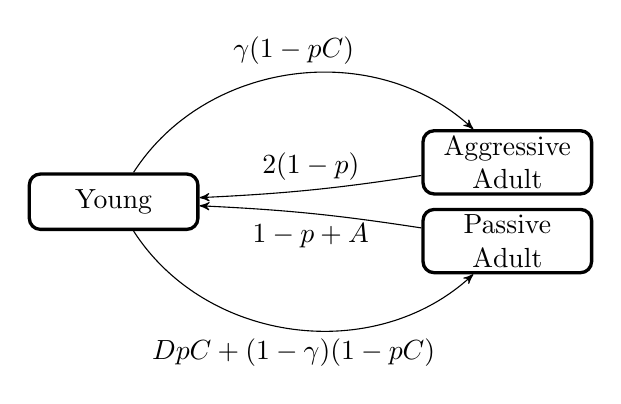
\begin{tikzpicture}[->,>=stealth']

    \node[state,anchor=center,text width=2cm]
        (Y) {Young};
    \node[state,anchor=center,text width=2cm,yshift=0.5cm,right of=Y,node distance=5.0cm]
        (A) {Aggressive\\Adult};
    \node[state,anchor=center,text width=2cm,yshift=-0.5cm,right of=Y,node distance=5.0cm]
        (P) {Passive\\Adult};

    \path (Y) edge[bend left=50]  node[anchor=south,above]{$\gamma(1-pC)$} (A);
    \path (A) edge[bend left=3]   node[anchor=south,above]{$2(1-p)$} (Y);
    \path (P) edge[bend left=-3]   node[anchor=south,below]{$1-p+A$} (Y);
    \path (Y) edge[bend left=-50] node[anchor=south,below]{$DpC+(1-\gamma)(1-pC)$} (P);

\end{tikzpicture}
\end{center}
\caption{A diagram of the flow of individual organisms between states of a simple Hawk-Dove game\\$\gamma$ being strategy parameter between $G_\mathbf{a}$ and $G_\mathbf{b}$, $p$ being proportion of Adults that are Aggressive, and $A$,$D$,$C$ being game parameters}
\label{fig:flow}
\end{figure}

We compared the results of the python software (of section \ref{sec:implementation}) on the Hawk-Dove game with those obtained by mathematical analysis (as given in Appendix \ref{appendix3}) and also via stochastic simulation.

The Moran process is a very simple stochastic model of the evolution of finite populations, wherein each 'turn' a random individual is chosen for reproduction proportional to its fitness and a corresponding random individual is chosen for death, the Moran process is generally regarded as a cornerstone technique of stochastic evolutionary game dynamics.\cite{stochastic1}

A Moran process for the above game is programmed (with source-code shown in Appendix \ref{appendix4}) and the results of the Moran process against the python implementation and mathematical analysis are shown in figure \ref{fig:bigfigure}.
The figure shows the value $p$ (the proportion of adults that are aggressive) and the proportion of young ($\%Y$) at equilibrium against the parameter $A$ for fixed $C$ and $D$ and shows a strong coincidence in achieving a non-trivial result for all three methodologies.

\begin{figure}[]
\begin{center}
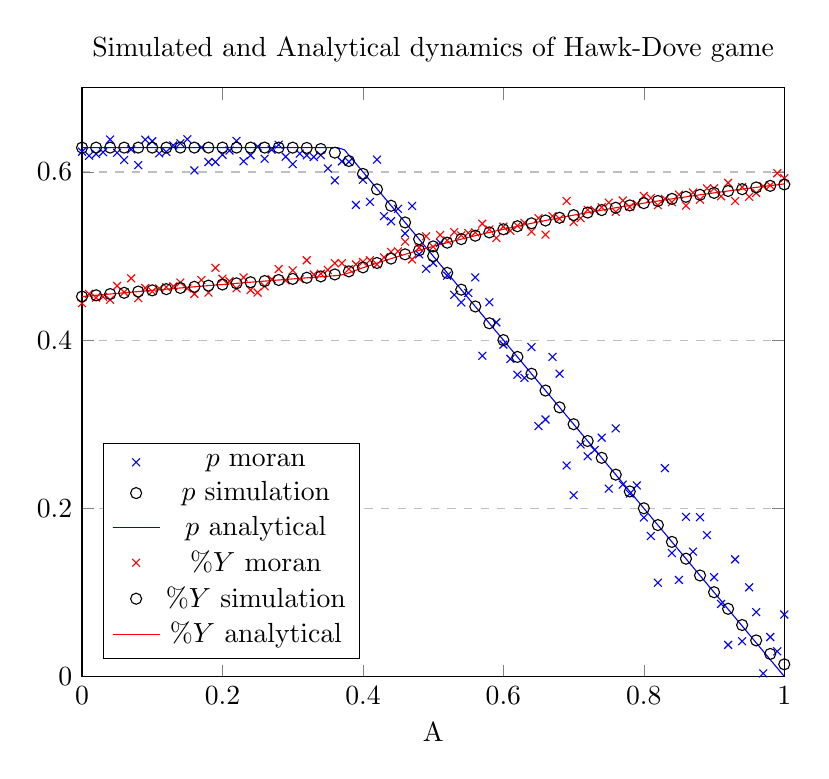
\begin{tikzpicture}
\begin{axis}[
    title={Simulated and Analytical dynamics of Hawk-Dove game},
    xlabel={A},
    xmin=0, xmax=1,
    ymin=0, ymax=0.7,
    xtick={0,0.2,0.4,0.6,0.8,1.0},
    ytick={0,0.2,0.4,0.6,0.8,1.0},
    legend pos=south west,
    ymajorgrids=true,
    grid style=dashed,
]
 
\addplot[
    color=blue,
    mark=x,
only marks,
    ]
    coordinates {
    (0.0,0.6241007194244604)(0.01,0.6192660550458715)(0.02,0.62147406733394)(0.03,0.6235186873290793)(0.04,0.6385869565217391)(0.05,0.6227824463118581)(0.06,0.6141804788213628)(0.07,0.6267806267806267)(0.08,0.6081818181818182)(0.09,0.6384758364312267)(0.1,0.6365313653136532)(0.11,0.6220984215413184)(0.12,0.6238361266294227)(0.13,0.6315298507462687)(0.14,0.6340545625587959)(0.15,0.6388115134633241)(0.16,0.6018348623853211)(0.17,0.6291390728476821)(0.18,0.6117755289788408)(0.19,0.6118677042801557)(0.2,0.6204933586337761)(0.21,0.6254716981132076)(0.22,0.6369545032497679)(0.23,0.6127497621313035)(0.24,0.6197964847363552)(0.25,0.6301747930082797)(0.26,0.6156716417910447)(0.27,0.6265402843601896)(0.28,0.6323957322987391)(0.29,0.6181474480151229)(0.3,0.6092843326885881)(0.31,0.6218009478672986)(0.32,0.6198019801980198)(0.33,0.617816091954023)(0.34,0.6199616122840691)(0.35000000000000003,0.6040658276863504)(0.36,0.5899705014749262)(0.37,0.6125860373647984)(0.38,0.612027158098933)(0.39,0.5607843137254902)(0.4,0.5907297830374754)(0.41000000000000003,0.5643564356435643)(0.42,0.6147058823529412)(0.43,0.5473579262213359)(0.44,0.5414141414141415)(0.45,0.5561172901921132)(0.46,0.5269151138716356)(0.47000000000000003,0.5595238095238095)(0.48,0.5020408163265306)(0.49,0.48478488982161594)(0.5,0.4918200408997955)(0.51,0.5157894736842106)(0.52,0.4766355140186916)(0.53,0.45387062566277836)(0.54,0.444794952681388)(0.55,0.4560846560846561)(0.56,0.4745762711864407)(0.5700000000000001,0.38136511375947996)(0.58,0.4450373532550694)(0.59,0.4211076280041797)(0.6,0.3946236559139785)(0.61,0.3776595744680851)(0.62,0.3588362068965517)(0.63,0.3550488599348534)(0.64,0.39171974522292996)(0.65,0.2978021978021978)(0.66,0.3055848261327713)(0.67,0.38011049723756907)(0.68,0.3600439077936334)(0.6900000000000001,0.2508630609896433)(0.7000000000000001,0.21545157780195864)(0.71,0.27582417582417584)(0.72,0.26179775280898876)(0.73,0.26936026936026936)(0.74,0.2839366515837104)(0.75,0.22336769759450173)(0.76,0.29497206703910617)(0.77,0.22811059907834103)(0.78,0.217440543601359)(0.79,0.2271689497716895)(0.8,0.18903150525087514)(0.81,0.16705336426914152)(0.8200000000000001,0.11149032992036405)(0.8300000000000001,0.24768518518518517)(0.84,0.14678899082568808)(0.85,0.11475409836065574)(0.86,0.18977272727272726)(0.87,0.14840989399293286)(0.88,0.18937644341801385)(0.89,0.16805721096543505)(0.9,0.11799761620977355)(0.91,0.08624708624708624)(0.92,0.03753026634382567)(0.93,0.13924050632911392)(0.9400000000000001,0.041866028708133975)(0.9500000000000001,0.10593713620488941)(0.96,0.07647058823529412)(0.97,0.0035971223021582736)(0.98,0.046875)(0.99,0.029887920298879204)(1.0,0.0736196319018405)
    };
\addlegendentry{$p$ moran}
\addplot[
    color=black,
    mark=o,
only marks,
    ]
    coordinates {
(0,0.6289575466)(0.02,0.6289575466)(0.04,0.6289575466)(0.06,0.6289575466)(0.08,0.6289575466)(0.1,0.6289575466)(0.12,0.6289575466)(0.14,0.6289575466)(0.16,0.6289575466)(0.18,0.6289575465)(0.2,0.6289575451)(0.22,0.6289575318)(0.24,0.6289574112)(0.26,0.6289564175)(0.28,0.6289490304)(0.3,0.6289001852)(0.32,0.6286217323)(0.34,0.6273346255)(0.36,0.622964624)(0.38,0.6130200741)(0.4,0.5976515858)(0.42,0.5792825877)(0.44,0.5597835311)(0.46,0.539932344)(0.48,0.5199776121)(0.5,0.4999921004)(0.52,0.4799970362)(0.54,0.4599988331)(0.56,0.4399995329)(0.58,0.4199998251)(0.6,0.3999999577)(0.62,0.3800000258)(0.64,0.360000069)(0.66,0.3400001064)(0.68,0.3200001504)(0.7,0.3000002138)(0.72,0.2800003163)(0.74,0.2600004944)(0.76,0.2400008227)(0.78,0.2200014619)(0.8,0.2000027757)(0.82,0.1800056245)(0.84,0.1600121288)(0.86,0.1400277109)(0.88,0.1200666434)(0.9,0.1001671363)(0.92,0.0804311295)(0.94,0.0611204033)(0.96,0.0428443188)(0.98,0.0267625127)(1,0.0143807301)
    };
\addlegendentry{$p$ simulation}
\addplot [
    domain=0:1, 
    samples=100, 
    color=blue,
    ]
    {min(1-x,(-1*(0.7+1)+sqrt((0.7+1)^2+4*(0.75*0.7-0.7)))/(2*(0.75*0.7-0.7)))};
\addlegendentry{$p$ analytical}

\addplot[
    color=red,
    mark=x,
only marks,
    ]
    coordinates {
    (0.0,0.444)(0.01,0.455)(0.02,0.4505)(0.03,0.4515)(0.04,0.448)(0.05,0.4645)(0.06,0.457)(0.07,0.4735)(0.08,0.45)(0.09,0.462)(0.1,0.458)(0.11,0.4615)(0.12,0.463)(0.13,0.464)(0.14,0.4685)(0.15,0.4615)(0.16,0.455)(0.17,0.4715)(0.18,0.4565)(0.19,0.486)(0.2,0.473)(0.21,0.47)(0.22,0.4615)(0.23,0.4745)(0.24,0.4595)(0.25,0.4565)(0.26,0.464)(0.27,0.4725)(0.28,0.4845)(0.29,0.471)(0.3,0.483)(0.31,0.4725)(0.32,0.495)(0.33,0.478)(0.34,0.479)(0.35000000000000003,0.4835)(0.36,0.4915)(0.37,0.4915)(0.38,0.4845)(0.39,0.49)(0.4,0.493)(0.41000000000000003,0.495)(0.42,0.49)(0.43,0.4985)(0.44,0.505)(0.45,0.5055)(0.46,0.517)(0.47000000000000003,0.496)(0.48,0.51)(0.49,0.5235)(0.5,0.511)(0.51,0.525)(0.52,0.5185)(0.53,0.5285)(0.54,0.5245)(0.55,0.5275)(0.56,0.528)(0.5700000000000001,0.5385)(0.58,0.5315)(0.59,0.5215)(0.6,0.535)(0.61,0.53)(0.62,0.536)(0.63,0.5395)(0.64,0.529)(0.65,0.545)(0.66,0.5255)(0.67,0.5475)(0.68,0.5445)(0.6900000000000001,0.5655)(0.7000000000000001,0.5405)(0.71,0.545)(0.72,0.555)(0.73,0.5545)(0.74,0.558)(0.75,0.5635)(0.76,0.5525)(0.77,0.566)(0.78,0.5585)(0.79,0.562)(0.8,0.5715)(0.81,0.569)(0.8200000000000001,0.5605)(0.8300000000000001,0.568)(0.84,0.564)(0.85,0.573)(0.86,0.56)(0.87,0.5755)(0.88,0.567)(0.89,0.5805)(0.9,0.5805)(0.91,0.571)(0.92,0.587)(0.93,0.5655)(0.9400000000000001,0.582)(0.9500000000000001,0.5705)(0.96,0.575)(0.97,0.583)(0.98,0.584)(0.99,0.5985)(1.0,0.5925)
    };
\addlegendentry{$\%Y$ moran}

\addplot[
    color=black,
    mark=o,
only marks,
    ]
    coordinates {
(0,0.4517891488)(0.02,0.4533007859)(0.04,0.4547950448)(0.06,0.4562723037)(0.08,0.4577329282)(0.1,0.4591772724)(0.12,0.4606056792)(0.14,0.4620184805)(0.16,0.4634159981)(0.18,0.4647985439)(0.2,0.4661664205)(0.22,0.467519924)(0.24,0.4688593629)(0.26,0.4701852059)(0.28,0.4714991067)(0.3,0.4728101081)(0.32,0.4741654624)(0.34,0.4757588605)(0.36,0.4780953866)(0.38,0.4817321369)(0.4,0.4865074548)(0.42,0.4917375503)(0.44,0.4969566765)(0.46,0.501998492)(0.48,0.5068270573)(0.5,0.5114452157)(0.52,0.5158650917)(0.54,0.5201001195)(0.56,0.52416307)(0.58,0.5280656464)(0.6,0.5318184805)(0.62,0.5354312238)(0.64,0.5389126531)(0.66,0.5422707686)(0.68,0.5455128809)(0.7,0.5486456873)(0.72,0.5516753368)(0.74,0.5546074882)(0.76,0.5574473581)(0.78,0.5601997623)(0.8,0.5628691478)(0.82,0.565459611)(0.84,0.567974887)(0.86,0.5704182752)(0.88,0.5727924)(0.9,0.5750985588)(0.92,0.5773350747)(0.94,0.5794935866)(0.96,0.5815525074)(0.98,0.583471595)(1,0.5852028369)
    };
\addlegendentry{$\%Y$ simulation}

\addplot [
    domain=0:1, 
    samples=100, 
    color=red,
    ]
    {max(sqrt(2*x)/(sqrt(2*x)+sqrt(0.7*(1-x)*(0.75-1)+1)), (sqrt(0.75*0.6289575465860742*0.7*(1+0.6289575465860742+x)))/(sqrt(0.75*0.6289575465860742*0.7*(1+0.6289575465860742+x))+1-0.6289575465860742*0.7+0.75*0.6289575465860742*0.7))};
\addlegendentry{$\%Y$ analytical}
 
\end{axis}
\end{tikzpicture}
\caption{Dynamics of the Hawk-Dove game across parameter $A$, with $D = 0.75$ and $C = 0.70$\\ shown are results for $p$ as well as proportion Young $\%Y$ for Moran stochastic simulation, analytical prediction, and our software solver's results}
\label{fig:bigfigure}
\end{center}
\end{figure}


\section{Discussion}\label{sec:discussion}

The game (as defined in section \ref{section:formalism}) is designed with broad features in an attempt to encapsulate a large number of potential applications.
The game's elements consist of there being a population/s of entities that can be described as stateful and stochastically transmit themselves between states based on their present state and the states and actions of others in accordance with a conserved strategy of choosing actions.

In a former version of this paper there was an objecting concern: how could the organisms of the simulation ever be responsive to the actions of the others?
If the strategy that is encoded into an organism determines what actions it will take based on its state alone, then how could that action ever change? And thence from this, how could the organisms even have the most basic intelligence?

It is a good question, and a tentative answer is by allowing to organisms to execute actions that are responsive to the actions of others.
Probably one of the most basic examples is the tit-for-tat strategy in the iterated prisoners dilemma, where the strategy changes the action played (cooperate or defect) based on the last play of the opponent. In appendix \ref{appendix:titfortat} we flesh out another example where a tit-for-tat-like strategy can be played by the organisms.

The approach involves the use of a binary state which could easily be interpreted as holding the 'memory' of the previous play, and allowing a set of actions which play cooperate/defect along with changing the state of the memory depending on the play of the opponent.
At this point it is good to note that the organisms in this example have an uncanny resemblance to Finite-State-Machines.

The primary breadth of the game's flexibility comes from allowing the transmission terms $T_{k,i,j}$ to be any function of population state $P^*_t$.\\
For instance, the $T$ terms can be non-linear and represent non-linear dynamics between individuals, such as might be potentially encoded in a classical evolutionary game with a 3-player symmetric payoff matrices. The $T$ terms might keep the total population size under a maximum, or only under a maximum or minimum for a particular state. And can be seen to encode dynamics similar to various evolutionary models eg. replicator dynamics, best-response dynamics or payoff comparison dynamics.\cite{psr1,errors1} It might be seen that the game's representation can be built to capture some of the dynamics of other evolutionary games.

Consideration must be made in running the game's simulation (per algorithm \ref{al:1}) that there is no guarantee it will fall into a stable equilibrium, or that it will do so in a timely manner. This is particularly true if astability is intrinsically part of the model (such as the game of paper-scissors-rock \cite{rockpaperscissors}). It is also worth noting that setting $\alpha$ too high can potentially introduce astability into borderline stable models.

A limitation of our game is that it is intentionally designed to 'wash-out' periodic transients between the states as the simulation progresses (as $\alpha<1$ acts as a dampener on such transients) so it cannot be used to model populations in which long-term periodic behavior between states in the simulation is desired\footnote{although $\alpha$ *could* be set to 1 to facilitate this}.
Another limitation is that there is no current facilitation for transmission of organisms from one strategy into another, such as might be used to explicitly model the effects of significant mutation on the population (see Nowak \cite{nowak} for example analysis) or also perhaps model the sexual combination of strategies.

However ultimately the features of evolutionary games and frameworks, with their virtues and shortcomings have to be evaluated and compared for some purpose.
And it is on this note that we must leave the game with its potential uses, limitations, and concepts unto the reader's imagination.



\vspace{6pt} 
\acknowledgments{}
\conflictsofinterest{The authors declare no conflict of interest. And the founding sponsors had no role in the design of the study; in the collection, analyses, or interpretation of data; in the writing of the manuscript, and in the decision to publish the results.} 

\appendixtitles{no}
\appendixsections{multiple}
\appendix
\section{That all proportionally present strategies have the same growth-rate at equilibrium}\label{appendix1}
At an equilibrium, if $m^{w^k}_{l,j}$ is the constant transmission matrix for strategy $w^k$, and if $v^{w^k,t}_j=P_{t,k,s_{k,j},w^k}$ is a vector of the number of organisms at time $t$ of strategy $w^k$ in the $j$th state.
Then application of the transmission matrix to the vector gives the vector at the next time index $t+1$ via Algorithm \ref{al:1} as:
$$ v^{w^k,t+1}_l=\alpha\left(\sum_jm^{w^k}_{l,j}v^{w^k,t}_j\right) + (1-\alpha)v^{w^k,t+1}_l ~~~~~~~~~~\text{ie.}~~~~~~~~~~v^{w^k,t+1} = \left(\alpha m^{w^k} + (1-\alpha)I\right)v^{w^k,t}$$
Thus the strategy's population vector $v^{w^k,t}$ can be stepped forward in time by repeated matrix multiplication by the non-negative matrix $Z = (\alpha m^{w^k} + (1-\alpha)I)$ where $I$ is identity matrix.\\
It is generally observed that repeated matrix powers often yields exponential growth and if we assume $Z$ is irreducible and diagonalisable matrix then the proof is straightforward and Theorem \ref{th:0} gives the desired result:
\begin{equation}\label{eq:growth}\lim_{m\rightarrow\infty}\frac{v^{w^k,t}}{(\alpha\lambda_{w^k}+(1-\alpha))^t}=b^{w^k}\hat{v}^{w^k}~~~~~~~~~~~\text{thus:}~~~~~~~~~~~v^{w^k,t}\approx(\alpha\lambda_{w^k}+(1-\alpha))^tb^{w^k}\hat{v}^{w^k}\end{equation}
Where $\lambda_{w^k}$ and $\hat{v}^{w^k}$ are largest eigenvalue and corresponding eigenvector of $m^{w^k}$, and $b^{w^k}$ is a constant.
If we assume the same is true for all strategies in the population then each has an asymptotic exponential growth-rate $\gamma_{w^k}=\alpha\lambda_{w^k}+1-\alpha$.
And so between any two strategies $w^k$ and $w^p$, that if $\lambda_{w^k}>\lambda_{w^p}$ then $\gamma_{w^k}>\gamma_{w^p}$ and strategy $w^k$ dominates strategy $w^p$.
Thus between the strategies in the population the only strategies that will be ultimately undominated are those of the maximum growth-rate.
And thus at equilibrium the only strategies of significant proportion in the population have the same growth-rate $\gamma$.
\\

The set of possible matrices $m^{w^k}$ (and $Z$) is obviously much larger than those diagonalisable and irreducible. And while is generally observed that most matrices yield the same exponential-growth character there are some which don't, specifically defective matrices\footnote{consider the linear growth of vector $\begin{bmatrix}1\\1\end{bmatrix}$ by repeated multiplications of matrix $\begin{bmatrix}1 & 1\\0 & 1\end{bmatrix} $}. In this paper we assume such matrices are the rare exception and our analysis does not treat their case. Although we believe that all conclusions of the paper hold with their case included it will be left to future (and more mathematically involved) work to demonstrate such.

\input{appendix2}
\pagebreak
\section{The Proofs}\label{appendix5b}

\begin{Lemma}\label{lem1}
for sets of complex numbers $\lambda_n$ and $\gamma_n$ related by $\gamma_n=\alpha\lambda_n+1-\alpha$ for an $\alpha$ such that $0<\alpha<1$ and $\lambda_0 = \max_n(|\lambda_n|)$ that: $\gamma_0=\max_n(|\gamma_n|)$ and for any $\gamma_m\ne\gamma_0$ that $|\gamma_m|<\gamma_0$ 
\end{Lemma}
\begin{proof}
Applying the triangle inequality for any $\lambda_m$:\\
$|\gamma_m|=|\alpha\lambda_m+1-\alpha|\le|\alpha\lambda_m|+|1-\alpha|=\alpha|\lambda_m|+1-\alpha$\\
Therefore:\\
$|\gamma_m|\le\alpha\max_n(|\lambda_n|)+1-\alpha=\alpha\lambda_0+1-\alpha=\gamma_0$\\
Hence $\gamma_0$ is upper bound for set $|\gamma_m|$ and also is identical to an element in the set, hence is a maxima; satisfying the first part of the proof.\\
For a $\gamma_m\ne\gamma_0$ then $\lambda_m\ne\lambda_0$, and we break $\lambda_m$ into real and imaginary components $\lambda_m=r_m+\mathbf{i}i_m$ (for $\mathbf{i}$ being imaginary number).\\
If $r_m>\lambda_0$ then $\sqrt{r^2_m+i^2_m}=|\lambda_m|>\lambda_0$ which is contradiction of construction of $\lambda_0$.\\
If $r_m=\lambda_0$ then $\sqrt{r^2_m+i^2_m}=|\lambda_0|\le\lambda_0$ would only be true if $i_m=0$, then $\gamma_m=\gamma_0$ contradicting construction of $\gamma_m$.\\
Therefore $r_m<\lambda_0$.\\
As $\gamma_m=\alpha\lambda_m+(1-\alpha)$ then:\\
$|\gamma_m|^2=(\alpha r_m+(1-\alpha))^2+(\alpha i_m)^2=\alpha^2(r_m^2+i_m^2)+2\alpha r_m(1-\alpha) + (1-\alpha)^2$\\
Since $|\lambda_m|\le\lambda_0$ therefore $r_m^2+i_m^2\le\lambda_0^2$, and also that $r_m<\lambda_0$:\\
$|\gamma_m|^2<\alpha^2\lambda_0^2+2\alpha \lambda_0(1-\alpha) + (1-\alpha)^2 = (\alpha\lambda_0 + (1-\alpha))^2=|\gamma_0|^2$\\
Therefore $|\gamma_m| < |\gamma_0|$, and the proof is complete.
\end{proof}



\begin{Theorem}\label{th:0}
for an irreducible, diagonalizable non-negative real $n\times n$ matrix $M$ with spectral radius $\lambda$, and non-negative non-zero vector $v$ and an $\alpha$ such that $1>\alpha>0$, then for $Z=(\alpha M+(1-\alpha)I)$.\\
That $\lambda$ is an eigenvalue of $M$ and its corresponding positive eigenvector $z$ is such there is an $b\in \mathbb{R_+}$ that: $$\lim_{m\rightarrow\infty}\frac{Z^mv}{(\alpha\lambda+(1-\alpha))^m}=bz$$
\end{Theorem}
\begin{proof}
Since $M$ is irreducible and non-negative then it has a non-negative real eigenvalue $\lambda_0$ equal to its spectral radius $\lambda$ and a corresponding positive eigenvector $z_0$ via Perron-Frobenius theorem\footnote{that an irreducible matrix has an element-wise positive eigenvector corresponding to the eigenvalue equal to its spectral radius}.
Let $z_0,z_1,\dots$ and $\lambda_0,\lambda_1,\dots$ be set of complex eigenvectors/values for $M$ (vectors as scaled to have magnitude of 1), in which case $z_0,z_1,\dots$ and $\gamma_0,\gamma_1,\dots$ are eigenvectors/values for $Z$ with $\gamma_i=\alpha\lambda_i+(1-\alpha)$.\\
Since $\lambda_0=\lambda$, then $\gamma_0=\alpha\lambda_0+(1-\alpha)$ is unique largest magnitude eigenvalue of $Z$, as via lemma \ref{lem1}.\\
since $z_0,z_1,\dots$ span $\mathbb{C}^n$, therefore $v$ can be decomposed into a linear combination of them:\\
$v = c_0z_0 + c_1z_1 + c_2z_2 +\dots = \sum_i(v\boldsymbol{\cdot}z_i)z_i~~~~~\text{(where $\boldsymbol{\cdot}$ is hermitian inner product)}$\\
With $c_0,c_1,\dots$ being the complex coefficients. Because vector $v$ is non-negative and non-zero and $z_0$ is also positive therefore $c_0$ is real and positive.
Taking $m$ repeated applications of $\frac{1}{\gamma_0}Z$ gives:\\
$\frac{Z^mv}{\gamma_0^m} = \left(\frac{\gamma_0}{\gamma_0}\right)^mc_0z_0 + \left(\frac{\gamma_{1}}{\gamma_0}\right)^mc_1z_1 + \left(\frac{\gamma_{2}}{\rho(Z)}\right)^mc_2z_2 + \dots$\\
for large $m$, all terms with $\gamma_{a_i}$ magnitudes less than that of $\gamma_0$ tend to zero leaving the single term:\\
$\frac{Z^mv}{\gamma_0^m} = \left(\frac{\gamma_0}{\gamma_0}\right)^mc_0z_0=c_0z_0$\\
therefore:\\
$\frac{Z^mv}{(\alpha\lambda_0+(1-\alpha))^m} = c_0z_0$\\
which completes the proof.
\end{proof}


\pagebreak





\begin{Lemma}\label{lem2}
for a $n\times n$ matrix $A$, and $n$ column vector $b$, with $A^{b,k}$ denoting the matrix with its $k$th column as $b$.
If $\lambda$ is an eigenvalue for both $A$ and $A^{b,k}$ then it is also an eigenvalue for $\alpha A + (1-\alpha)A^{b,k}$ for any $\alpha \in \mathbb{R}$
\end{Lemma}
\begin{proof}
Consider the characteristic polynomials of $\lambda$ for $A$ and $A^{b,k}$:\\
$\det(A-\lambda I)=\det(A^{b,k}-\lambda I)=0$\\
If we let $C(\cdot)_{i,j}$ denote the $i$,$j$th cofactor of a matrix, then these determinants can be expanded along the $k$th column to give:\\
$\left(\sum_iA_{i,k}C(A-\lambda I)_{i,k}\right)-\lambda C(A-\lambda I)_{k,k}=\left(\sum_ib_iC(A-\lambda I)_{i,k}\right)-\lambda C(A-\lambda I)_{k,k}=0$\\
Therefore:\\
$\alpha\left(\left(\sum_iA_{i,k}C(A-\lambda I)_{i,k}\right)-\lambda C(A-\lambda I)_{k,k}\right) + (1-\alpha)\left(\left(\sum_ib_iC(A-\lambda I)_{i,k}\right)-\lambda C(A-\lambda I)_{k,k}\right)=0$\\
$=\left(\sum_i(\alpha A_{i,k}+(1-\alpha)b_i)C(A-\lambda I)_{i,k}\right)-\lambda C(A-\lambda I)_{k,k} =\det(\alpha A + (1-\alpha)A^{b,k}-\lambda I)=0$\\
Thus it is demonstrated that $\lambda$ is also an eigenvalue for $\alpha A + (1-\alpha)A^{b,k}$.
\end{proof}

\begin{Theorem}\label{th:2}
For a real $n\times n$ element-wise non-negative matrix $A$, and real element-wise non-negative column vector $b$, with $A^{b,k}$ denoting the matrix with its $k$th column as $b$.
For the matrix mapping $B(\alpha) = \alpha A + (1-\alpha)A^{b,k}$ defined on a range $0\le\alpha\le1$. If $\rho(B(\alpha))$ denotes the spectral radius of $B(\alpha)$.\\ Then $\rho(B(\alpha))$ is continuous, and either constant or strictly monotonic with $\alpha$.
\end{Theorem}
\begin{proof}
Because $B(\alpha) = \alpha A + (1-\alpha)A^{b,k}$ is a matrix continuous in all its elements it is thus well established that it will have $n$ continuous eigenvalues\cite{matrix1}.\footnote{An informal outline of the proof is that: 1. If the elements of a matrix are continuous 2. Then the coefficients of the characteristic polynomial are continuous (as they are additions and multiplications of them) 3. Then the roots of the characteristic polynomial are continuous (see \cite{roots1}) 4. Hence the eigenvalues are continuous}\\
It is thus straightforward to note that the function $\rho(B(\alpha))$ is also continuous with $\alpha$ for all $\alpha$.\\
Furthermore that the value $\rho(B(\alpha))$ is itself an eigenvalue of $B(\alpha)$ for all $\alpha$ via the Perron-Frobenius theorem\footnote{\label{note1}that an element-wise non-negative matrix has an eigenvalue equal to its spectral radius. The proof of this one seems quite difficult to find even though it certainly is stated in literature (for instance \cite{bo1}). Furthermore it also something which might be seem as intuitive, as any non-negative matrix can be constructed as the limit of a sequence of element-wise positive matricies and as the eigenvalues of a matrix must be continuous on their elements, thus that the corresponding property should also hold in the limit.}.
Suppose for a contradiction that $\rho(B(\alpha))$ is not monotone, in this case there must exist at least three values of alpha, $\alpha_1<\alpha_2<\alpha_3$ such that $\rho(B(\alpha_2))>\max(\rho(B(\alpha_0)),\rho(B(\alpha_3)))$ or $\rho(B(\alpha_2))<\min(\rho(B(\alpha_0)),\rho(B(\alpha_3)))$.
\begin{itemize}[leftmargin=*,labelsep=4mm]
\item	suppose that $\rho(B(\alpha_2))>\max(\rho(B(\alpha_1)),\rho(B(\alpha_3)))$: let $\beta$ be a value between $\rho(B(\alpha_2))$ and $\max(\rho(B(\alpha_1)),\rho(B(\alpha_3)))$. Thus via the intermediate value theorem there exists $\gamma_1$ ($\alpha_1<\gamma_1<\alpha_2$) and $\gamma_2$ ($\alpha_2<\gamma_2<\alpha_3$) such that $\rho(B(\gamma_1))=\rho(B(\gamma_2))=\beta$. Thus $\beta$ is an eigenvalue of $B(\alpha_1)$ (via Lemma \ref{lem2}), and $\beta > \rho(B(\alpha_1))$ which contradicts the construction of $\rho(B(\alpha_1))$.
\item   suppose that $\rho(B(\alpha_2))<\min(\rho(B(\alpha_1)),\rho(B(\alpha_3)))$: let $\beta$ be a value between $\rho(B(\alpha_2))$ and $\min(\rho(B(\alpha_1)),\rho(B(\alpha_3)))$. Thus via the intermediate value theorem there exists $\gamma_1$ ($\alpha_1<\gamma_1<\alpha_2$) and $\gamma_2$ ($\alpha_2<\gamma_2<\alpha_3$) such that $\rho(B(\gamma_1))=\rho(B(\gamma_2))=\beta$. Thus $\beta$ is an eigenvalue of $B(\alpha_2)$ (via Lemma \ref{lem2}), and $\beta > \rho(B(\alpha_2))$ which contradicts the construction of $\rho(B(\alpha_2))$.
\end{itemize}
Therefore $\rho(B(\alpha))$ is monotonic.\\
If there does not exist any $\alpha_1,\alpha_2\in[0,1]$ such that $\rho(B(\alpha_1))$ = $\rho(B(\alpha_2))$\\
\-\hspace{8mm}then $\rho(B(\alpha))$ is strictly monotonic.\\
If there does exist an $\alpha_1,\alpha_2\in[0,1]$ such that $\rho(B(\alpha_1))$ = $\rho(B(\alpha_2))$\\
\-\hspace{8mm}then $\rho(B(\alpha))$ is constant via lemma \ref{lem2}.\\
Which completes the proof.
\end{proof}

\pagebreak

\begin{Theorem}\label{th:3}
For a $n\times n$ matrix $A_{i,j}$, and column vectors $b$ and $c$, with $A^{b,k}$ and $A^{c,k}$ denoting the matrix with its $k$th column as $b$ and $c$ respectively. For the matrix mapping $B(\alpha) = \alpha A^{b,k} + (1-\alpha)A^{c,k}$ for $\alpha\in\mathbb{R}$. Let $\lambda(\alpha)$ and $v(\alpha)$ be an eigenvalue/vector pairing of $B(\alpha)$\\
If there exists different $\alpha_1$ and $\alpha_2$ such that $\lambda(\alpha_1)=\lambda(\alpha_2)$, then $\lambda(\alpha)=\lambda(\alpha_1)$ and $v(\alpha)=\frac{\alpha-\alpha_1}{\alpha_2-\alpha_1}v(\alpha_2)+\frac{\alpha-\alpha_2}{\alpha_1-\alpha_2}v(\alpha_1)$ is an eigenvalue/vector pairing for all $\alpha$, with the $k$th value of the eigenvector - $v(\alpha)_k$ being constant.
\end{Theorem}
\begin{proof}
if $b=c$ then $A^{b,k}=A^{c,k}$ and $B(\alpha) = A^{b,k}$, then $\lambda(\alpha)=\lambda(\alpha_1)$ and $v(\alpha)=v(\alpha_1)$ is trivial solution which fulfills the proof. Otherwise $b\ne c$.\\
Since $\lambda(\alpha_1)$ is an eigenvalue for all $B(\alpha)$ via Lemma \ref{lem2} then $\frac{\partial \lambda(\alpha)}{\partial \alpha}=0$ and $\lambda(\alpha)=\lambda(\alpha_1)=\lambda$ is true.\\
As: $~\left(\alpha A^{b,k} + (1-\alpha)A^{c,k}\right)v(\alpha)=\lambda v(\alpha)$\\
If $v(\alpha)_k$ denotes the $k$th value of $v(\alpha)$, then differentiating with respect to $\alpha$ \\
Gives: $\left(\alpha A^{b,k} + (1-\alpha)A^{c,k} - \lambda I\right)\frac{\partial v(\alpha)}{\partial\alpha}+(b-c)v(\alpha)_k=0$\\
now, there are two cases:\\
if there is an $\alpha_3$ such that $v(\alpha_3)_k=0$ then:\\
\-\hspace{8mm}$\left(\alpha_3 A^{b,k} + (1-\alpha_3)A^{c,k} - \lambda I\right)\frac{\partial v(\alpha_3)}{\partial\alpha}=0$\\
\-\hspace{8mm}Setting $\frac{\partial v(\alpha)}{\partial\alpha}=0$ is permissible, making $v(\alpha)_k=0$.\\
\-\hspace{8mm}therefore constant $v(\alpha)=v(\alpha_3)$ is solution which fulfills the proof\\
if there is not an $\alpha_3$ such that $v(\alpha_3)_k=0$, then:\\
\-\hspace{8mm}It is possible do scaling, thus setting $v(\alpha)_k=d$ to be a non-zero constant and therefore $\frac{\partial v(\alpha)_k}{\partial \alpha}=0$\\
\-\hspace{8mm}Thus there is a $\frac{\partial v(\alpha)}{\partial\alpha}$ such that: $\left(\alpha A^{b,k} + (1-\alpha)A^{c,k} - \lambda I\right)\frac{\partial v(\alpha)}{\partial\alpha}+d(b-c)=0$\\
\-\hspace{8mm}Thus there is a $\frac{\partial v(\alpha)}{\partial\alpha}$ such that for all $i$: $\left(\sum_{j,j\ne k}\left(A_{i,j}-\lambda I_{i,j}\right)\frac{\partial v(\alpha)_j}{\partial\alpha}\right) +d(b_i-c_i)=0 $\\
\-\hspace{8mm}Therefore $\frac{\partial v(\alpha)}{\partial\alpha}$ can be constant\\
\-\hspace{8mm}Therefore $v(\alpha)=\frac{\alpha-\alpha_1}{\alpha_2-\alpha_1}v(\alpha_2)+\frac{\alpha-\alpha_2}{\alpha_1-\alpha_2}v(\alpha_1)$ is only linear solution that adjoins $v(\alpha_2)$ and $v(\alpha_2)$.\\
Which completes the proof.
\end{proof}



\begin{Theorem}\label{th:4}
For a real $n\times n$ element-wise non-negative matrix $A$, 
for $m$ element-wise non-negative column vectors $b_0,b_1,\dots$, 
for $A^{b_i,k}$ denoting the matrix with its $k$th column as $b_i$, 
for the matrix mapping $B(c_0,c_1,\dots) = \sum_{i}c_iA^{b_i,k}$ defined on inputs where: $\forall i~c_i\ge 0$ and $\left(\sum_{i=0}^{m-1}c_i\right)=1$, 
for $\rho(B)$ denoting the spectral radius of $B$, 
for $V(\cdot,\lambda)_k$ denoting the $k$th element of an eigenvector of a matrix corresponding to eigenvalue $\lambda$, 
for a set of reals $d_0,d_1,\dots$: 
$$\text{If:}~~~~~~~\rho(B(d_0,d_1,\dots)) = \max\rho(B)=\lambda ~~~~~~~\text{then:}~~~~~~~ $$ 
$$ V(B(d_0,d_1,\dots),\lambda) = \sum_{i=0}^{m-1}d_iV(A^{b_i,k},\lambda) ~~~~~~~\text{and:}~~~~~~~ $$
$$ \forall d_i\ne 0~~~~ V(A^{b_i,k},\lambda)_k=V(B(d_0,d_1,\dots),\lambda)_k=C  ~~~~\text{ie. they all have the same kth value, equal C}$$
\end{Theorem}
\begin{proof}
We begin by introducing the following mapping on the coordinates $c_0,c_1,\dots,c_{m-1}$ by parameter $\alpha$, valid for $0\le\alpha\le 1$ and $c_{m-1}\ne 1$:\\
\inlineequation[eq:part2]{Q(c_0,c_1,\dots,c_{m-1},\alpha)=B\left(\frac{c_0(1-\alpha)}{\sum_{y=0}^{m-2}c_y},\frac{c_{1}(1-\alpha)}{\sum_{y=0}^{m-2}c_y},\dots,\frac{c_{m-2}(1-\alpha)}{\sum_{y=0}^{m-2}c_y},\alpha\right)=\alpha A^{b_{m-1},k} + (1-\alpha)\frac{\sum_{y=0}^{m-2}c_yA^{b_y,k}}{\sum_{y=0}^{m-2}c_y}}\\
$Q$ is a valid mapping under the input constraints, Ie. that the inputs to $B$ satisfy the constraints if the $c$-inputs of $Q$ (the $c_0,c_1,\dots,c_{m-1}$) satisfy the constraints (that they are non-negative and they sum to one).
We also notice by inspection of equation \ref{eq:part2} that $Q(\dots,\alpha)$ satisfies the criteria for Theorem \ref{th:2} and thus $\rho(Q(\dots,\alpha))$ is either constant or strictly monotonic.
When $\alpha=1$ the input to $B$ takes the singular value: \inlineequation[eq:part5]{Q(c_0,c_1,\dots,c_{m-1},1)=B(0,0,\dots,1)=A^{b_{m-1},k}}\\
When $\alpha=0$ the input to $B$ takes the zero of the last value with the other values scaled to validate input constraints: \\\inlineequation[eq:part6]{Q(c_0,\dots,c_{m-1},0)=B(\gamma c_0,\dots,\gamma c_{m-2},0)=B(\gamma c_0,\dots,\gamma c_{m-2}) ~~~~~~~~\text{with:}~~~~~~~~ \gamma = (\sum_{i=0}^{m-2}c_i)^{-1}}\\
And when $\alpha=c_{m-1}$ that \inlineequation[eq:part7]{Q(c_0,c_1,\dots,c_{m-1},c_{m-1})=B(c_0,c_1,\dots,c_{m-1})}\\
Proof by induction:
\begin{itemize}[leftmargin=*,labelsep=4mm]
\item	Considering the case $m=1$: In which case there is a singular vector $b_0$ and the only permissible value of $B(d_0)$ under the constraints is $B(1)$ therefore $V(B(d_0),\lambda) = V(A^{b_0,k},\lambda)$ thus the theorem is satisfied for $m=1$.
\item   Considering the case $m=j+1$ under the assumption of theorem satisfaction of $m=j$:\\
\-\hspace{4mm}If $d_j=1$ then:\\
\-\hspace{8mm}$V(B(d_0,d_1,\dots),\lambda) = V(A^{b_j,k},\lambda)$ and the theorem is satisfied\\
\-\hspace{4mm}Otherwise:\\
\-\hspace{8mm}$\rho(Q(d_0,d_1,\dots,d_{j},\alpha))$ exists and is constant or strictly monotonic with $\alpha$\\
\-\hspace{8mm}- as per theorem \ref{th:2} on equation \ref{eq:part2}\\
\-\hspace{8mm}$\rho(Q(d_0,d_1,\dots,d_{j},\alpha))$ passes through $\rho(B(d_0,d_1,\dots,d_{j}))$\\
\-\hspace{8mm}- as per equation \ref{eq:part7}.\\
\-\hspace{8mm}Assuming $\rho(B(d_0,d_1,\dots,d_{j}))\ge\max(\rho(Q(c_0,c_1,\dots,c_{j},1)), \rho(Q(c_0,c_1,\dots,c_{j},0)))$\\
\-\hspace{8mm}- which is a condition of the theorem.\\
\-\hspace{8mm}If $\rho(Q(d_0,d_1,\dots,d_{j},\alpha))$ is strictly monotonic then it must be maximal at \\
\-\hspace{8mm}either side $\alpha=0$ or $\alpha=1$ or otherwise it must be constant, thus there are three cases:\\
\-\hspace{12mm}If $d_j=1$ then $\rho(B(d_0,d_1,\dots,d_{j}))=\rho(Q(c_0,c_1,\dots,c_{j},1))$:\\
\-\hspace{16mm}Then $V(B(d_0,d_1,\dots),\lambda) = V(A^{b_j,k},\lambda)$ and the theorem is satisfied\footnote{this line is technically redundant, but is included for an \dots attempt\dots at logial flow.}\\
\-\hspace{12mm}If $d_j=0$ then $\rho(B(d_0,d_1,\dots,d_{j}))=\rho(Q(c_0,c_1,\dots,c_{j},0))$: \\
\-\hspace{16mm}Then $B(d_0,d_1,\dots,d_{j-1},d_{j})=B(d_0,d_1,\dots,d_{j-1})$\\
\-\hspace{16mm}And $V(B(d_0,d_1,\dots,d_{j-1},d_{j}),\lambda) = V(B(d_0,d_1,\dots,d_{j-1}),\lambda)$\\
\-\hspace{16mm}And $V(B(d_0,d_1,\dots,d_{j-1}),\lambda) = \sum_{i=0}^{m-2}d_iV(A^{b_i,k},\lambda)$\\
\-\hspace{16mm}- by the inductive assumption\\
\-\hspace{16mm}Thus $V(B(d_0,d_1,\dots,d_{j-1},d_{j}),\lambda) = \sum_{i=0}^{m-1}d_iV(A^{b_i,k},\lambda)$ and the theorem is satisfied\\
\-\hspace{12mm}Otherwise $\rho(Q(d_0,d_1,\dots,d_{j},\alpha)) $ must remain constant with any change in $\alpha$:\\
\-\hspace{16mm}Since $Q(d_0,d_1,\dots,d_{j},\alpha)$ is non-negative matrix\\
\-\hspace{16mm}Then $\rho(Q(d_0,d_1,\dots,d_{j},\alpha))=\lambda$ is an eigenvalue of it\\
\-\hspace{16mm}-via the Perron-Frobenius theorem\footnote{see footnote \ref{note1}}\\
\-\hspace{16mm}Thus via Theorem \ref{th:3}:\\
\-\hspace{16mm}$V(Q(d_0,d_1,\dots,d_{j},\alpha),\lambda)$\\
\-\hspace{22mm}$ = \alpha V(Q(d_0,d_1,\dots,d_{j},1),\lambda) + (1-\alpha) V(Q(d_0,d_1,\dots,d_{j},0),\lambda)$\\
\-\hspace{16mm}and $V(Q(d_0,d_1,\dots,d_{j},\alpha),\lambda)_k=C$ is constant irrespective of $\alpha$\\
\-\hspace{16mm}So doing immediate substitutions from equations \ref{eq:part5},\ref{eq:part6},\ref{eq:part7}:\\
\-\hspace{16mm}$V(B(d_0,d_1,\dots,d_{j}),\lambda)$\\
\-\hspace{22mm}$ = d_j V(A^{b_j,k},\lambda) + (1-d_j) V(B(\gamma d_0,\gamma d_1,\dots,\gamma d_{j-1}),\lambda) ~~~~\text{with:}~~~~\gamma = (\sum_{i=0}^{j-1}d_j)^{-1}$\\
\-\hspace{16mm}And $V(B(d_0,d_1,\dots,d_{j}),\lambda)_k=V(A^{b_j,k},\lambda)_k=V(B(\gamma d_0,\gamma d_1,\dots,\gamma d_{j-1}),\lambda)_k=C$\\
\-\hspace{16mm}As $V(B(\gamma d_0,\gamma d_1,\dots,\gamma d_{j-1}),\lambda) = \gamma\sum_{i=0}^{m-2}d_iV(A^{b_i,k},\lambda)$\\
\-\hspace{16mm}- by the inductive assumption\\
\-\hspace{16mm}and each non-zero $d_i$ has $V(A^{b_i,k},\lambda)_k=C$\\
\-\hspace{16mm}Thus: $V(B(d_0,d_1,\dots,d_{j}),\lambda) = \sum_{i=0}^{m-1}d_iV(A^{b_i,k},\lambda)$ and the theorem is satisfied
\end{itemize}
Which completes the proof.
\end{proof}


\pagebreak

\begin{Theorem}\label{th:5}
For $n$ sets of real element-wise non-negative $n$-column vectors, $\{y_{0,0},y_{0,1},\dots,y_{1,0},y_{1,1},\dots\}$.\\
Letting $q$ be similarly dimensioned set of sets of real numbers, $q=\{q_{0,0},q_{0,1},\dots,q_{1,0},q_{1,1},\dots\}$\\
Letting $q^{\{i,j\}}$ be the same as $q$ except modified in that the subset $q_i$ is all zeros except for the $j$th being 1.\\ 
Letting $q^{\{i,j\},a,b,c\dots}$ be the same as $q^{\{i,j\}}$ except that the first unmodified subset is all zeros except for the $a$th being $1$, and the second unmodified $q$ subset is all zeros except for the $b$th, and etc.\\
Considering matrix constructions of form: \\
$m(a) = 
\left[\begin{array}{c|c|c|c}
\sum_{x}a_{0,x}y_{0,x} & 
\sum_{x}a_{1,x}y_{1,x} & 
\sum_{x}a_{2,x}y_{2,x} & \dots
\end{array}\right]$\\
Defined for any $a$ input such that: $\forall j~\sum_{i}a_{j,i}=1$ and $\forall j,i~~a_{j,i}\ge 0$.\\
for $\rho(\cdot)$ is spectral radius, and $V(\cdot,\lambda)$ is an eigenvector of a matrix for eigenvalue $\lambda$, and $\delta$ is Kronecker delta.\\
If $\rho(m(q)) = \max_\zeta\rho(m(\zeta))=\lambda$\\
Then
$$ \forall i,j~~V(m(q),\lambda)_jq_{j,i} = \sum_k\sum_\alpha\dots\sum_\omega q_{0,\alpha}\dots q_{n-1,\omega}V(m(q^{\{j,k\},\alpha,\beta,\gamma,\dots,\omega}),\lambda)_j\delta_{ik} $$
\end{Theorem}

\begin{proof}$~$\\
For any $j$, Theorem \ref{th:4} applies to $m(q)$ on the $j$th set of $q$'s values:\\
Therefore $V(m(q),\lambda)=\sum_i q_{j,i}V(m(q^{\{j,i\}}),\lambda)$ and $\forall i:q_{j,i}\ne 0\Rightarrow~~V(m(q^{\{j,i\}}),\lambda)_j=C$ is a constant.\\
Thus $V(m(q),\lambda)_j=\sum_i q_{j,i}V(m(q^{\{j,i\}}),\lambda)_j=\sum_i q_{j,i}C=C$, and\\
Therefore $\forall i:q_{j,i}\ne 0\Rightarrow~~V(m(q),\lambda)_j=V(m(q^{\{j,i\}}),\lambda)_j$\\
Thus $\forall i~~q_{j,i}V(m(q),\lambda)_j= q_{j,i}V(m(q^{\{j,i\}}),\lambda)_j$\\
Thus \inlineequation[eq:part8]{\forall i~~q_{j,i}V(m(q),\lambda)_j= \sum_k\delta_{ik}q_{j,k}V(m(q^{\{j,k\}}),\lambda)_j}\\
\\
Now, theorem \ref{th:4} applies to $V(m(q^{\{j,k\}}),\lambda)$:\\
therefore $V(m(q^{\{j,k\}}),\lambda) = \sum_\alpha q_{0,\alpha}V(m(q^{\{j,k\},\alpha}),\lambda)$\\
theorem \ref{th:4} applies again to to $V(m(q^{\{j,k\},\alpha}),\lambda)$:\\
therefore $V(m(q^{\{j,k\},\alpha}),\lambda) = \sum_\beta q_{1,\beta}V(m(q^{\{j,k\},\alpha,\beta}),\lambda)$\\
theorem \ref{th:4} applies again to to $V(m(q^{\{j,k\},\alpha,\beta}),\lambda)$:\\
therefore $V(m(q^{\{j,k\},\alpha,\beta}),\lambda) = \sum_\gamma q_{2,\gamma}V(m(q^{\{j,k\},\alpha,\beta,\gamma}),\lambda)$\\
and so on$\dots$\\
Therefore: \inlineequation[eq:part9]{V(m(q^{\{j,k\}}),\lambda) = \sum_\alpha\sum_\beta\sum_\gamma\dots\sum_\omega q_{0,\alpha}q_{1,\beta}q_{2,\gamma}\dots q_{n-1,\omega}V(m(q^{\{j,k\},\alpha,\beta,\gamma,\dots,\omega}),\lambda)}\\
Which is fully expanded.\\
\\
Substituting equation \ref{eq:part9} into equation \ref{eq:part8} gives:\\
$\forall i~~q_{j,i}V(m(q),\lambda)_j = \sum_\alpha\sum_\beta\sum_\gamma\dots\sum_k\dots\sum_\omega q_{0,\alpha}q_{1,\beta}q_{2,\gamma}\dots q_{j,k}\dots q_{n-1,\omega}\delta_{ik}V(m(q^{\{j,k\},\alpha,\beta,\gamma,\dots,\omega}),\lambda)_j$\\
\\
Which completes the proof
\end{proof}

\pagebreak
\section{Derivation of Hawk-Dove dynamics}\label{appendix3}

The Hawk-Dove game given in the body of the article is simple enough to yield analytic solution.
It is possible to directly determine the largest real eigenvalue of the tranmsission matrix (as per equation \ref{eq:hd_transmission}) as: $$ \lambda = \sqrt{2\gamma(1-p)(1-pC)+(1-p+A)(DpC+(1-\gamma)(1-pC))} $$
And by this, it is posible to compute the equilibrium points of the population. The population's equilibrium points will either be on the 'interior' of the strategy space ($1>\gamma >0$) or be on the boundary ($\gamma=1$ or $\gamma=0$).
We can calculate the interior equilibrium points via the 'indifference principle'\cite{markov5}, whereby the population has reached an 'interior' equilibrium where it makes no more sense to play Dove any more than Hawk. This corresponds to the case where all Dove and Hawk strategies have the same growth-rate.

\subsection{the interior case for $1>\gamma >0$}

Solving for $\frac{\partial \lambda}{\partial \gamma}=0$ gives $$ 1-p=A $$ As the conditions for interior equilibrium.  This condition which corresponds to the Aggressive and Passive Adults having the same expected number of offspring.
Thus the expected population growth-rate at equilibrium is thus $$\lambda_{\{p=1-A\}} = \sqrt{2A}\sqrt{C(1-A)(D-1)+1}$$ This identifies that the total growth-rate is the multiplication of the roots of transmission rate from young to adult and from adult to young.\\
Using the shorthand: $P_Y=P^*_{t,b,\mathbf{y},G_{\mathbf{a}}}+P^*_{t,b,\mathbf{y},G_{\mathbf{p}}}$, and $P_A=P^*_{t,b,\mathbf{a},R_{\mathbf{a}}}$, and $P_P=P^*_{t,b,\mathbf{p},R_{\mathbf{p}}}$\\
The corresponding eigenvector of population proportions is (presented unnormalised for simplicity) as:

$$ \begin{bmatrix}
    P_Y \\
    P_A \\
    P_P \\
\end{bmatrix} = \begin{bmatrix}
    \lambda_{\{p=1-A\}} \\
    \gamma(1-C+CA) \\
    DC(1-A) + (1-\gamma)(1-C+CA) \\
\end{bmatrix} $$

Thus the fraction of Child to Adults at equilibrium is $\frac{P_Y}{P_Y+P_A+P_P} = \frac{\sqrt{2A}}{\sqrt{2A}+\sqrt{C(1-A)(D-1)+1}}$

\subsection{the boundary case for $\gamma=1$}

The growth-rate of strategy $\gamma=1$ is $\lambda_{\{\gamma=1\}}=\sqrt{2(1-p)(1-pC)+DpC(1-p+A)}$ and has population proportions:
$$ \begin{bmatrix}
    P_Y \\
    P_A \\
    P_P \\
\end{bmatrix} = \begin{bmatrix}
    \lambda_{\{\gamma=1\}} \\
    1-pC \\
    DpC  \\
\end{bmatrix}$$

A population of $\gamma=1$ (in which $p=\frac{P_A}{P_A+P_P}$) has $p=\frac{-(C+1)+\sqrt{(C+1)^2+4(DC-C)}}{2(DC-C)}$ (which exists if $(C+1)^2+4(DC-C)>0$).
The strategy $\gamma=1$ is strictly dominant strategy when all other strategies have a lower growth-rate:
$$\forall\gamma ~~~~ \lambda_{\{\gamma=1,p=\dots\}}^2 > \lambda_{\{p=\dots\}}^2$$
$$\forall\gamma ~~~~ 2(1-p)(1-pC)+(1-p+A)DpC > 2\gamma(1-p)(1-pC)+(1-p+A)(DpC+(1-\gamma)(1-pC))$$
$$\forall\gamma ~~~~ 1-p-A > \gamma(1-p-A)$$

which is true iff $p < 1-A$, which thus happens on a condition among the $A,C,D$: 

$$ \sqrt{(C+1)^2+4(DC-D)} > 2(1-A)(DC-D)+C+1 $$

When this condition is met, the strategy $\gamma=1$ dominates, yielding $p=\frac{-(C+1)+\sqrt{(C+1)^2+4(DC-C)}}{2(DC-C)}$ with the fraction of Child to Adults $\frac{P_Y}{P_Y+P_A+P_P} = \frac{\sqrt{DpC(1+p+A)}}{\sqrt{DpC(1+p+A)}+1-pC+DpC}$

\subsection{the boundary case for $\gamma=0$}

The growth-rate of strategy $\gamma=0$ is $\lambda_{\{\gamma=0\}}=\sqrt{(1-p-A)(DpC+1-pC)}$ and has population proportions:
$$ \begin{bmatrix}
    P_Y \\
    P_A \\
    P_P \\
\end{bmatrix} = \begin{bmatrix}
    \lambda_{\{\gamma=0\}} \\
    0 \\
    DpC+1-pC  \\
\end{bmatrix}$$
A population of $\gamma=0$ (in which $p=\frac{P_A}{P_A+P_P}$) has straightforwardly $p=0$ and growth-rate $\lambda_{\{\gamma=0,p=0\}}=\sqrt{1-A}$.

However, in such a population the strategy $\gamma=1$ has a greater growth-rate than $\gamma=0$ as: $\left(\lambda_{\{\gamma=1,p=0\}} = \sqrt{2}\right) > \left(\sqrt{1-A} = \lambda_{\{\gamma=0,p=0\}}\right)$
and thus the boundary case $\gamma=0$ is never an dominant strategy.

\subsection{Stitching it together}

Given the parameters of the game $A,C,D$ is: $$(C+1)^2+4(DC-D)>0 ~~~~~~~\text{and}~~~~~~~ \sqrt{(C+1)^2+4(DC-D)} > 2(1-A)(DC-D)+C+1 ~~~~~~~\text{?} $$
\begin{itemize}[leftmargin=*,labelsep=3mm]
\item	if so then the Game equilibrium is Hawk-Saturated:$$p=\frac{-(C+1)+\sqrt{(C+1)^2+4(DC-C)}}{2(DC-C)}~~~~~~\text{and}~~~~~~~\frac{P_Y}{P_Y+P_A+P_P} = \frac{\sqrt{DpC(1+p+A)}}{\sqrt{DpC(1+p+A)}+1-pC+DpC}$$
\item	if not then a Hawk-Dove equilibrium exists:$$p=1-A~~~~~~\text{and}~~~~~~~\frac{P_Y}{P_Y+P_A+P_P} = \frac{\sqrt{2A}}{\sqrt{2A}+\sqrt{C(1-A)(D-1)+1}}$$
\end{itemize}


\pagebreak
\input{appendix5}

\bibliography{./bib}
\end{document}

